% СПО ЛКС - TCP/IP
% Пынькин Д.А. (с) 2011
\documentclass[ignorenonframetext, hyperref={pdftex, unicode}]{beamer}
\usepackage{beamerthemesplit}

\usetheme{Pittsburgh}
\usecolortheme{dolphin}

\usepackage[russian]{babel}
\usepackage[utf8]{inputenc}
\usepackage[T1]{fontenc}
\usepackage{ulem}
%\usepackage{html}

\usepackage{verbatim}

\usepackage{tikz}
\usetikzlibrary{positioning,arrows}

\title[СПОЛКС (http://goo.gl/32cTB)]{Системое программное обеспечение локальных компьютерных сетей}
\author{Денис Пынькин}
\date{2011 -- 2012}
%\institution[БГУИР]{Белорусский государственный университет информатики и радиоэлектроники}
%\logo{
\includegraphics[width=1cm]{logo-kafEVM.png}}


\subtitle[TCP/IP]{Стек протоколов TCP/IP\\(Продолжение)}

\begin{document}

\mode<all>{\begin{frame}
\titlepage
\begin{center}
e-mail: denis.pynkin@bsuir.by\\
\end{center}
\begin{center}
{\bfseries http://goo.gl/32cTB}

{\tiny СЧАСТЬЕ ДЛЯ ВСЕХ, ДАРОМ, И ПУСТЬ НИКТО НЕ УЙДЕТ ОБИЖЕННЫЙ!\\
(c)Стругацкие, Пикник на обочине}
\end{center}
\end{frame}
}

%
% Далее начинается сама презентация
%

\section{ARP}

\begin{frame}{ARP}
	\begin{block}{ARP -- Address Resolution Protocol\\протокол определения адреса}
		использующийся в компьютерных сетях протокол низкого уровня,  предназначенный для определения адреса канального уровня по известному адресу сетевого уровня.
	\end{block}
\end{frame}


\begin{frame}{ARP: протокол определения адреса}
	Сетевой интерфейс имеет аппаратный адрес (48-битное значение для Ethernet или Token ring). 
Фреймы,  которыми обмениваются на аппаратном уровне,  должны адресоваться к корректному интерфейсу. 
Однако TCP/IP использует собственную схему адрессации: 32-битные IP адреса. 
Знание IP адреса хоста не позволяет ядру послать датаграмму этому хосту.\\
Драйвер Ethernet должен знать аппаратный адрес пункта назначения,  чтобы послать туда данные. В задачу ARP входит обеспечение динамического соответствия между 32-битными IP адресами и аппаратными адресами,  используемыми различными сетевыми технологиями.
\end{frame}

\begin{frame}{Принцип работы}
	\begin{enumerate}
		\item Узел,  которому нужно выполнить отображение IP-адреса на локальный адрес,  формирует ARP запрос,  вкладывает его в кадр протокола канального уровня,  указывая в нем известный IP-адрес,  и рассылает запрос широковещательно.
		\item Все узлы локальной сети получают ARP запрос и сравнивают указанный там IP-адрес с собственным.
		\item В случае их совпадения узел формирует ARP-ответ,  в котором указывает свой IP-адрес и свой локальный адрес и отправляет его уже направленно,  так как в ARP запросе отправитель указывает свой локальный адрес.
	\end{enumerate}
\end{frame}

\begin{frame}{ARP кэш}
	Эффективность функционирования ARP во многом зависит от ARP кэша (ARP cache),  который присутствует на каждом хосте.\\
	В кэше содержатся Internet адреса и соответствующие им аппаратные адреса.\\
	Стандартное время жизни каждой записи в кэше составляет 2 минуты с момента создания записи.
\end{frame}

\begin{frame}[fragile]{Пример просмотра ARP-кэша}
\scriptsize
	\begin{verbatim}
# arp -a
host1 (10.0.0.113) at 00:0f:fe:d4:e6:bb [ether] on eth0
host2 (10.0.0.15) at 78:e3:ff:94:63:58 [ether] on eth0
host3 (10.0.0.1) at 00:2f:29:35:03:7c [ether] on eth0
host4 (10.0.0.8) at 00:15:45:0e:2f:82 [ether] on eth0
	\end{verbatim}
\normalsize
\end{frame}

\section{Протоколы транспортного уровня}

\begin{frame}{Порт}
	\begin{block}{Порт протокола транспортного уровня}
	идентифицируемый номером системный ресурс,  выделяемый приложению,  выполняемому на некотором сетевом хосте,  для связи с приложениями,  выполняемыми на других сетевых хостах (в том числе c другими приложениями на этом же хосте).
	\end{block}
\end{frame}
\begin{frame}{Для чего нужны порты?}
	Порты необходимы по двум причинам:
	\begin{enumerate}
		\item используются как идентификатор для разделения траспортных сессий между одинаковыми оконечными точками
		\item используются для идентификации протокола прикладного уровня и ассоциированного с ним сервиса
	\end{enumerate}
\end{frame}
\begin{frame}{1 порт = 16 бит}
Для каждого из протоколов TCP и UDP стандарт определяет возможность одновременного выделения на хосте до 65536 уникальных портов,  идентифицирующихся номерами от 0 до 65535.\\
	\pause
	{\bfseries Порты TCP не пересекаются с портами UDP. То есть,  порт 1234 протокола TCP не будет мешать обмену по UDP через порт 1234!!!}
\end{frame}

\begin{frame}{Диапазоны портов}
	http://www.iana.org/assignments/service-names-port-numbers/service-names-port-numbers.xml:\\
	\begin{itemize}
		\item Системные (0-1023)
		\item Пользовательские (1024-49151)
		\item Динамические и/или частные (49152-65535)
	\end{itemize}
	\bigskip
	{\bfseries Для большинства ОС системный диапазон доступен только с привилегиями администратора!}
\end{frame}

\subsection{UDP}
\begin{frame}{UDP -- User Datagram Protocol}
Протокол UDP (RFC-768) является одним из основных протоколов,  расположенных непосредственно над IP. Он предоставляет прикладным процессам транспортные услуги,  немногим отличающиеся от услуг протокола IP.\\
\bigskip
Протокол UDP обеспечивает доставку дейтограмм,  но не требует подтверждения их получения. Протокол UDP не требует соединения с удаленным модулем UDP ("бессвязный" протокол)
\end{frame}

\begin{frame}{Формат дейтаграммы UDP}
	\begin{center}
		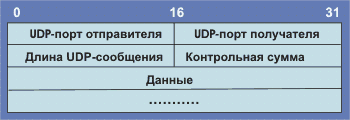
\includegraphics[width=0.9\textwidth]{04-udp_header.png}
	\end{center}
	Длина включает в себя заголовок.\\
	Контрольная сумма рассчитывается с использованием псевдозаголовка!
\end{frame}

\begin{frame}{Контрольная сумма}
Контрольная сумма с использованием псевдозаголовка необходима как защита от дейтаграмм, ошибочно направленных по другому адресу.
	\begin{center}
		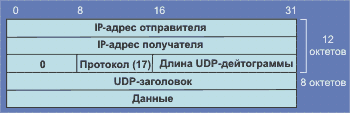
\includegraphics[width=0.5\textwidth]{04-udp_pseudoheader.png}
	\end{center}
Контрольная сумма UDP не является обязательной. Если она не подсчитывается,  ее значение равно 0 (настоящая нулевая контрольная сумма кодируется всеми единицами).
\end{frame}

\subsection{TCP}
\begin{frame}{TCP -- RFC-793}
	\begin{block}{TCP -- Transmission Control Protocol}
		Это {\itshape надежный} протокол {\itshape с установлением соединений}, позволяющий без ошибок 
		доставлять {\itshape байтовый поток} с одной машины на любую другую машину объединенной сети.
		Он разбивает входной поток байтов на отдельные сообщения и передает их межсетевому уровню. 
		В пункте назначения этот протокол собирает из полученных сообщений выходной поток. 
		Кроме того,  TCP осуществляет управление потоком.
	\end{block}
\end{frame}

\begin{frame}{Механизмы надежности TCP}
	\begin{itemize}
		\item Контрольная сумма -- позволяет определить повреждение данных и/или заголовка TCP-сегмента.
		\item Определение дублирующихся сегментов -- "дубли" выкидываются.
		\item Повторная передача -- используются подтверждения о доставке данных. Отсутствие подтверждений вместе с механизмом таймеров приводит к повторной передаче данных.
		\item Корректная последовательность -- TCP собирает сегменты в правильном порядке.
		\item Таймеры -- позволяют управлять повторной передачей сегментов.
	\end{itemize}
\end{frame}


\begin{frame}{Формат пакета TCP}
	\begin{center}
		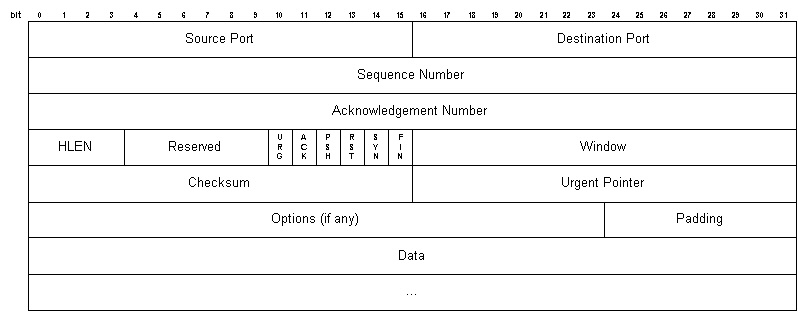
\includegraphics[width=1\textwidth]{04-tcp_header.png}
	\end{center}
	\tiny
	HLEN -- длина заголовка в 32-хбитных словах. В RFC обозначается, как "data offset"\\
	window -- указывает отправителю, сколько данных получатель готов принять\\
	Urgent pointer -- указывает смещение октета, следующего за срочными данными, относительно первого октета
	\normalsize
\end{frame}

\begin{frame}{Поле Flags}
	\begin{itemize}
		\item Urgent Pointer (URG)
		\item Acknowledgement (ACK)
		\item Push Function (PSH)
		\item Reset the Connection (RST)
		\item Synchronize (SYN)
		\item No More Data from Sender (FIN)
	\end{itemize}
\end{frame}

\begin{frame}{Поле Options}
	\begin{itemize}
		\item End of Option List
		\item No-Operation
		\item Maximum Segment Size
		\item WSOPT - Window Scale
		\item SACK
		\item много дополнительных опций
	\end{itemize}
\end{frame}


\begin{frame}{Установка соединения TCP}
	\begin{center}
		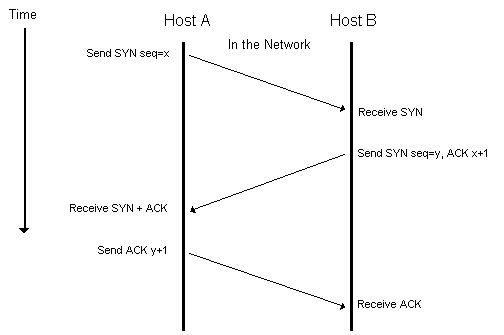
\includegraphics[height=0.5\textheight]{04-tcp-connection-establishment.png}
	\end{center}
\end{frame}

\begin{frame}{Разрыв соединения TCP}
	\begin{center}
		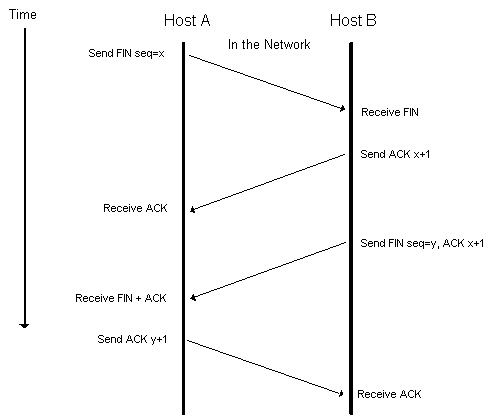
\includegraphics[height=0.7\textheight]{04-tcp-connection-termination.png}
	\end{center}
\end{frame}

\begin{frame}{Управление потоком с помощью скользящего окна}
	\begin{center}
		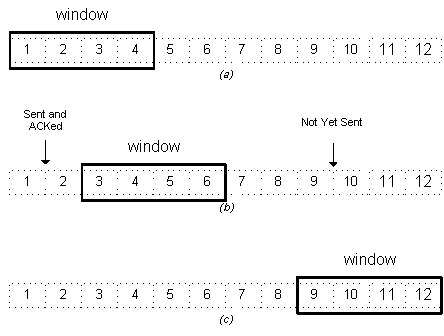
\includegraphics[height=0.7\textheight]{04-sliding-window.png}
	\end{center}
\end{frame}

\begin{frame}{Управление насыщением -- механизм медленного старта}
	Congestion Control:
	\begin{itemize}
		\item Slow Start -- с каждой успешной передачей размер буфера удваивается до половины точки насыщения-- далее по 1 сегменту. Вплоть до размера окна.
		\item Congestion Avoidance -- противовес медленному старту. Уменьшает размер окна в 2 раза,  но не менее 2 сегментов. В случае таймаута -- уменьшается до 1 сегмента и запускается механизм медленного старта.
	\end{itemize}
\end{frame}

\begin{frame}[fragile]{Алгоритм Нэгла(Nagle)}
Борется с неэффективной передачей.
\begin{verbatim}
if there is new data to send
  if the window size >= MSS and available data is >= MSS
      send complete MSS segment now
  else
    if there is unconfirmed data still in the pipe
      enqueue data in the buffer until an acknowledge is received
    else
      send data immediately
    end if
  end if
end if
\end{verbatim}
\end{frame}



\begin{frame}{Синдром узкого окна}
Такого рода проблема возникает в том случае,  когда данные поступают отправителю крупными блоками,  а интерактивное приложение адресата считывает информацию побайтно.\\
\bigskip
\pause
Кларк предложил не посылать уведомление о ненулевом значении ширины окна при считывании одного байта,  а лишь после освобождения достаточно большого пространства в буфере. Например,  когда адресат готов принять MSS байтов или когда буфер наполовину пуст.
\end{frame}


\begin{frame}{Таймеры ТСР}
	\begin{itemize}
		\item Таймер повторных передач (retransmission; RTO) -- для сегмента
		\item Таймер запросов (persist timer) -- для 0-го окна
		\item Таймер контроля работоспособности (keepalive)
		\item 2MSL-таймер (Maximum Segment Lifetime) -- время в состоянии TIME\_WAIT
	\end{itemize}

\end{frame}

\begin{frame}[fragile]{Пример статистики TCP соединений}
	\tiny
	\begin{verbatim}
# netstat -antp
Active Internet connections (servers and established)
Proto Recv-Q Send-Q Local Address       Foreign Address             State       PID/Program name   
tcp        0      0 0.0.0.0:45803       0.0.0.0:*                   LISTEN      6184/rpc.mountd     
tcp        0      0 127.0.0.1:631       0.0.0.0:*                   LISTEN      6048/cupsd          
tcp        0      0 192.168.0.1:56734   74.125.77.189:443           ESTABLISHED 23679/xulrunner     
tcp        0      0 192.168.0.1:56724   74.125.77.189:443           TIME_WAIT   -                   
tcp        0      0 192.168.0.1:48176   69.171.241.10:5222          ESTABLISHED 10931/telepathy-gab 
tcp        0      0 ::1:631             :::*                        LISTEN      6048/cupsd          
	\end{verbatim}
	\normalsize
\end{frame}

\begin{frame}{Диаграмма состояний TCP}
	\begin{center}
		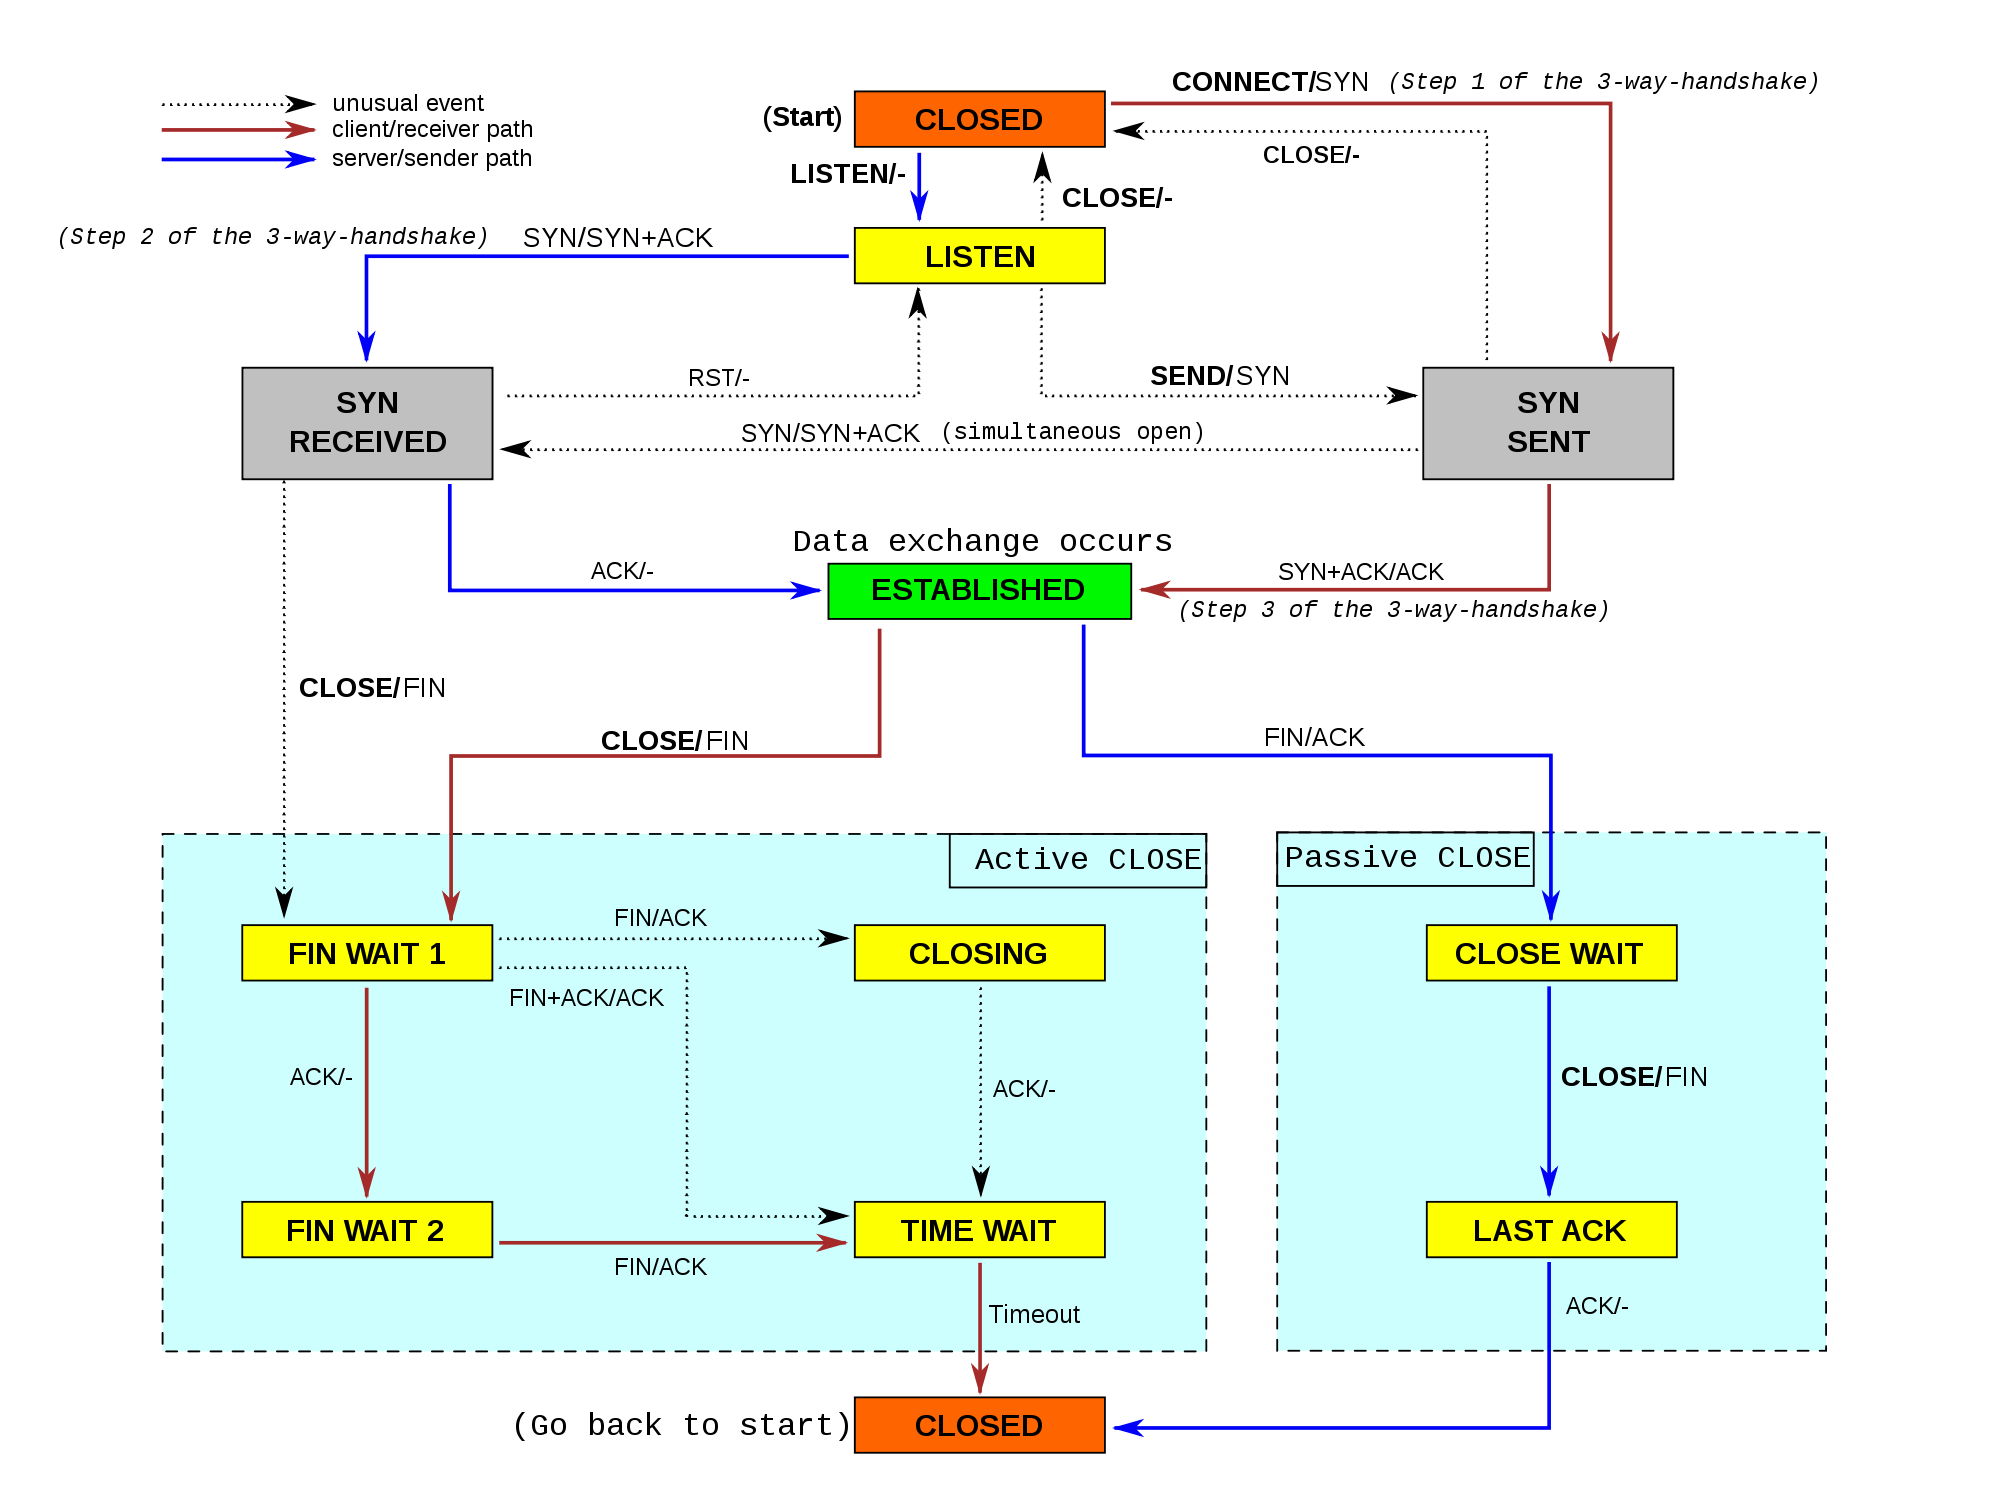
\includegraphics[height=0.8\textheight]{04-2000px-Tcp_state_diagram.png}
	\end{center}
\end{frame}


\mode<all>{\begin{frame}{}
\Huge
\begin{center}
	Спасибо за внимание!
	\bigskip
	Вопросы?
\end{center}
\normalsize
\end{frame}
}

\end{document}
%Конец файла
